\documentclass[10pt,a4paper,UTF8,fleqn]{article}
%\usepackage[utf8]{inputenc}
\usepackage{array,multirow,color,amsmath,amsfonts,amssymb}
\usepackage{graphicx,booktabs,geometry,fancyhdr,listings,xcolor,bm,multicol,float}
\usepackage[colorlinks %linkcolor=black, anchorcolor=black, citecolor=black,filecolor=black,urlcolor=black
 ]{hyperref}
\usepackage[center,tiny,]{titlesec}
\usepackage{subfig}   % 使用子图形
\usepackage{indentfirst} % 中文段落首行缩进
\usepackage{bm}          % 公式中的粗体字符(用命令\boldsymbol)
\usepackage{multicol}    % 正文双栏
\usepackage{indentfirst} % 中文首段缩进
\usepackage{abstract}    % 2栏文档,一栏摘要及关键字宏包
\usepackage{amsthm}      % 使用定理
\usepackage{siunitx}
\usepackage{upgreek}
\usepackage{tikz,xcolor,eso-pic}
\usepackage{times}
\usepackage{wasysym}
\usepackage{pifont}
\usepackage[sort]{cite}
\usepackage{float}
\usepackage{lettrine}
\usepackage[perpage,bottom,stable,symbol*,splitrule,flushmargin]{footmisc}

\newcommand{\watermark}[3]{\AddToShipoutPictureBG{
		\parbox[b][\paperheight]{\paperwidth}{
			\vfill%
			\centering%
			\tikz[remember picture, overlay]%
			\node [rotate = #1, scale = #2] at (current page.center)%
			{\textcolor{gray!80!cyan!15}{#3}};
			\vfill}}}

%\usepackage{blindtext}


\geometry{left=1.5cm,right=1.3cm,top=2.3cm,bottom=2cm,headsep=0.4cm}
\pagestyle{fancy}

%\setlength{\columnsep}{5mm}
%\setlength{\columnseprule}{0.01mm}
\begin{document}
%	\watermark{60}{10}{DRAFT}
%	\clearpage
%	\blinddocument
	\renewcommand{\thefootnote}{\roman{footnote}}
	\title{Synthesis of the Pierce Gun} 
	\date{}
	\author{\small J. RODNEY M. VAUGHAN, \footnotesize SENIOR MEMBER, IEEE}
	
	\renewcommand\thesection{\Roman{section}%\hspace{-0.5em}
	}
	\captionsetup[figure]{labelfont={small},textfont=%{bf,it}
		%normalfont
		,name={Fig.},labelsep=period%,justification=centering
	}
\twocolumn[\maketitle]

\small \textit{Abstract---}The design of a Pierce gun is uniquely defined by four parameters: beam voltage, current, waist radius, and cathode current density. The gun convergence angle, cathode spherical radius, anode-cathode spacing, and throw (distance to the waist) are calculated by an iterative procedure which typically converges in four cycles to \ang{0.1}.The anode lens formula of Danielson, Rosenfeld, and Saloom is combined with inverted forms of the Langmuir-Blodgett solution for the spherical diode and the Universal Beam Spread equation for the tunnel region; the iterations match the trajectories at the anode plane. Correction for spherical aberration is made by the method of Frost and Purl as quantified by True. The inverted equations are simple enough to be solved in a few minutes with a programmable calculator. The experimental data of Frost and Purl is used to demonstrate the validity of the procedure for guns of medium perveance.\footnotetext{Manucript recevied March 11, 1980; revised Angust 4, 1980.\\The author is with Linear Beam Department, Electron Tube Division, Litton Industries, San Carlos, CA 94070.}

%\let\thefootnote\relax\footnote[1]{Manucript recevied March 11, 1980; revised Angust 4, 1980.\\The author is with Linear Beam Department, Electron Tube Division, Litton Industries, San Carlos, CA 94070.}


%\textbf{Index:} H-plane and E-plane loads, slow-wave structure (SWS), terahertz (THz), traveling-wave tube (TWT).
%\vspace*{25pt}
\normalsize
\section{\textsc{Background}}

\lettrine[lines=2]{T}{HE DESIGN} of Pierce guns [1] has been based on graphical methods even up to quite recent times [2]. It has also proceeded on the basis of assuming an electrode configuration and finding the exit beam it would produce: if this is not the desired beam, then somewhat intuitive adjustments are made to the configuration until an acceptable beam is produced, first on paper and then in a beam tester.

The microwave tube designer would, of course, prefer a synthesis procedure, by which he can specify the beam he wants and calculate the configuration needed to produce it, any iterations needed in the calculation must be purely mechanical convergence procedures which do not depend on the designer's tuition. In this paper, such a synthesis procedure will be derived.

\renewcommand{\thefootnote}{\arabic{footnote}}
\section{\textsc{Input Parameters}}
The primary requirements, set by the tube (klystron or TWT) in which the gun is to be used, are the beam voltage, current, and diameter. The ``beam diameter'' is identified with the waist diameter (2$ r_w $, Fig.\ref{fig1}) of the gun: if the beam is caught by an appropriate magnetic field at this point, it will continue into the interaction region as a substantially parallel flow. Thus it is desirable to know the Position of the waist---the ``throw'' of the gun---in order to locate the magnetic field entrance correctly. Even if an ``immersed flow'' gun is to be used, a conventional (shielded) design is needed as a starting point.

A fourth parameter can be assigned, and for this we choose the cathode current density $ J_c $, because it is closely related to the desired life. The value chosen will depend on the kind of emitter (oxide coated or matrix, etc.) and on the operating conditions (CW or pulsed, etc.); even though there are no hard-and-fast relations determining the life. it seems better to have direct control of this parameter than to allow it to become the indirect result of other parameters.

The four quantities, $ V,I, r_w, $ and $ J_c $, define a unique Pierce gun (or no real design if an incompatible set is chosen). \textit{The convergence angle is no longer a free parameter}, but will be one of the results of the calculation: in fact, we shall use it as the parameter to be adjusted to obtain convergence of the solution.
\begin{figure}[t]
	\centering
	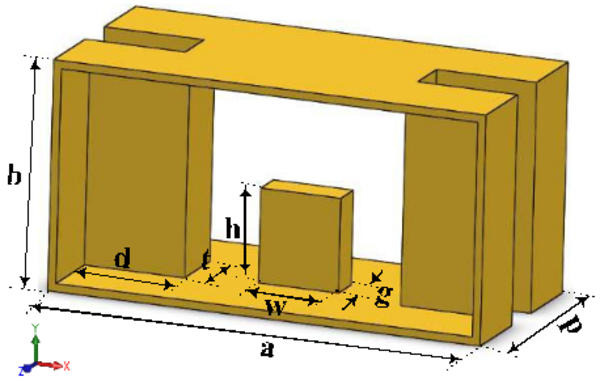
\includegraphics[width=0.99\linewidth]{figure/fig1}
	\caption{\small Pierce gun showing parameters used in the uncorrected design.}
	\label{fig1}
\end{figure}

\vspace{2ex}\textit{A. Outputs}\vspace{0.5ex}

The outputs needed to represent a basic gun design are the convergence half angle $ \theta $, the cathode disc and spherical radii $ r_c $ and $ R_c $, the anode-cathode spacing $ z_a $, the radius of the anode aperture $ r_a $, and the throw $ z_w $. Ancillary outputs will be the perveance $ \mu P $, the radius $ R_a $ of the equivalent anode sphere, and the beam radius at the anode plane $ r_b(z_a) $. The focus electrode is assumed to conform to Pierce's theory, making an angle of \ang{67.5} with the normal at the cathode edge.

\section{\textsc{Calculation}}
\textit{A. The Region From the Cathode to the Anode}\vspace{0.5ex}

The cathode disc radius can be obtained immediately as 
\begin{equation}
	r_c = (I/\pi J_c)^{1/2}
\end{equation}
and the microperveance as
\begin{equation} \label{eq:2}
	\mu P = 10^6 I/V^{3/2}.
\end{equation}
We now assign an initial estimate of $ 30\sqrt{\mu P} $ degree to $ \theta $. The error in this does not matter as long as it is not so large that the iterative calculation of $ \theta $ fails to converge, because the process is self-correcting. The expression easily given meets this requirement, at least out to \ang{70} half angle.

For each approximation to $ \theta $, we find Langmuir and Blodgett's parameter ($ -\varpropto $) from the formula given by Pierce [1,p.183, eq.(10.12) rearranged]
\begin{equation} \label{eq:3}
	(-\varpropto)^2 = 14.67(1-\cos\theta)/\mu P.
\end{equation}
Now $ L $ and $ B $ express $ -(\varpropto) $ in terms of a variable $ \gamma $, which in turn is a function of the spherical radii $ R_c $ and $ R_a $
\begin{equation} \label{eq:4}
	\gamma = \ln(R_c/R_a).
\end{equation}
$ (-\varpropto) $ is then given by the series
\begin{equation} \label{eq:5}
	\begin{split}
	(-\varpropto) = &\gamma + 0.3\gamma^2 + 0.075\gamma^3 + 0.01432\gamma^4 + 0.00216\gamma^5 \\&+ 0.00027\gamma^6.
	\end{split}
\end{equation}
The accuracy of this formula is improved if the last coefficient is changed to 0.00035, and it is then valid within 1 percent for $ R_c/R_a$ as high as 20--far larger than we need, and larger than Langmuir hirmself apparently realized. Since it is $ -(\varpropto) $ that we know from \eqref{eq:3}, we invert this equation by numerical methods and obtain
\begin{equation} \label{eq:6}
	\gamma = -(\varpropto) - 0.275(-\varpropto)^2 + 0.06(-\varpropto)^3 - 0.006(-\varpropto)^4.
\end{equation}
This equation does not cover as wide a range as \eqref{eq:5}, but it gives $ R_c/R_a $ within 1 percent up to $ -(\varpropto) = 2.8 $, correspondin to $ R_c/R_a \simeq 5$, which is still adequate for microwave tube guns he error is 2 percent at $ -(\varpropto) = 3.4, R_c/R_a \simeq 6$, and falls off rapidly thereafter: so this equation is inapplicable for extreme low-perveance high-convergence cases.

Obtaining $ \gamma$ from \eqref{eq:6} and, inverting \eqref{eq:4} we have
\begin{equation} \label{eq:7}
	R_c/R_a = e^\gamma
\end{equation}
and
\begin{align} \label{eq:8}
	r_b(z_a) &= r_c(R_a/R_c)\nonumber \\ &= r_ce^{-\gamma}
\end{align}

\vspace{0.5ex}\textit{B. Refraction at the Anode}\vspace{0.5ex}
 
For the effect of the anode lens. Pierce used the Davisson and Calbick [3] formula. Danielson, Rosenfeid, and Saloom [4] (D, R, and S hereafter) made a more detailed analysis including the effects of space-charge and thermal-emission velocities. Neglecting the thermals, their formula for the slope $ \phi_1 $ just to the right of the anode plane is
\begin{equation} \label{eq:9}
	\tan\phi_1 = \frac{r_c}{R_c}\left\lbrace 1- \Gamma r_b\left(z_a\right)\cdot\frac{R_c}{4\left(-\varpropto\right)^{4/3}R_a^2} \cdot \frac{d\left(\varpropto\right)^{4/3}}{d\left(R_c/R_a\right)}\right\rbrace
\end{equation}
Where $ \Gamma $ is D, R, and S's arbitrary correction factor which we set to $ 1.25 $. D, R, and S used the value 1.1, but the higher value in combination with True's Correction, to be discussed later, is found to give the best overall agreement with observation. The differential in \eqref{eq:9} is found in series from \eqref{eq:5}; substituting in \eqref{eq:9}, we then have
\begin{equation}\label{eq:10}
	\begin{split} 
	\tan\phi_1 = &\sin\theta\left\lbrace\right. 1-0.417\left(\right. 1+0.6\gamma+0.225\gamma^2+0.0573\gamma^3  \\ &+0.0108\gamma^4 + 0.0021\gamma^5 \left.\right) /\left(-\varpropto \right)\left. \right\rbrace 
	\end{split}
\end{equation}

in which all the quantities on the right have been determined by the inputs and the current trial value of $ \theta $. The factor 0.417 is $ (1.25)(1/4)(3/4) $.

\vspace{2ex}\textit{C. The Tunnel Region}\vspace{0.5ex}

Reverting to \eqref{eq:8}, we can now express the normalized compression $ R $ from the anode plane to the waist as
\begin{equation} \label{eq:11}
	R = r_b(z_a)r_w.
\end{equation}
Still neglecting thermals, the beam motion in this region is given by the ``Universal Beam Spread'' curves [5]; as normally presented this gives R in terms of $ Z $, but we can invert it to
\begin{equation}\label{eq:12}
\begin{split} 
Z = &11.0\left(R-1\right)^{0.5} + 1.32\left(R-1\right) + 0.0615\left(R-1\right)^2\\&-0.00167\left(R-1\right)^3 
\end{split}
\end{equation}
where
\begin{equation} \label{eq:13}
	Z = \left(z_w - z_a\right)\sqrt{\mu P}/r_w.
\end{equation}
Equation \eqref{eq:12} is valid within 1 percent for $ 1.01<R<20 $. We can also express the slope at normalized radius $ R $ by the formula [5, p.284]\footnote{equation \eqref{eq:14} is confusing --- by translator(Li Shengming).}
\begin{equation} \label{eq:14}
	\begin{aligned}
	\tan\phi_2 =& \left(10^{-6}\mu P\cdot\ln R/2\pi\epsilon_0\sqrt{2\eta}\right)^{1/2}\\=&\cdot 17409\left(-\mu P\cdot\ln R\right)^{1/2}.
	\end{aligned}
\end{equation}


\vspace{0.5ex}\textit{D. Convergence to Half Angle $ \theta $}\vspace{0.5ex}

We now have two expressions, \eqref{eq:10} and \eqref{eq:14}, for the slope for the trajectory immediately to the right of the anode plane. For continuity of the trajectory, these must be brought to equality by adjustment of $ \theta $. An effective procedure is simply to multiply the prior value of $ \theta $ by $(\tan \phi_2/\tan\phi_1)^{1/2}$ and recalculate \eqref{eq:3} through \eqref{eq:14}. The interations\footnote{{may be iterations}} are stopped when $(\tan \phi_2/\tan\phi_1)^{1/2}$ falls within $ 1.0\pm0.005 $, which corresponds roughly to $ \pm\ang{0.1} $ in $ \theta $. Even on a programmable calculator (TI 59), each iteration can be completed in less than 15\,s; no more than four iterations have been needed in any cases tested,except the combination of very low perveance and high convergence.

\vspace{2ex}\textit{E. Completion of the Pierce Design}\vspace{0.5ex}


When $ \theta $ has been found to the desired accuracy, we obtain the remaining gun configuration parameters from

\begin{align}
	R_c = &r_c/\sin\theta \label{eq:15}\\
	R_a = &R_ce^{-\gamma} \label{eq:16}\\
	r_b(z_a) = &r_c e^{-\gamma} \label{eq:17}\\
	r_a = &1.2r_b(z_a) \label{eq:18}\\
	z_{ac} = &R_c - R_a \label{eq:19}\\
	z_a = & R_c - \sqrt{R_a^2 - r_a^2} \label{eq:20} \\
	z_w = & z_{ac} + r_w Z/\sqrt{\mu P} \label{eq:21}
\end{align}
where $ z_w $ is the throw from cathode vertex to waist, and $ Z $ is given by \eqref{eq:12}. The 1.2 factor in \eqref{eq:18} is an arbitrary clearance factor for the anode hole; a smaller hole may cause some anode interception, while a larger one will increase the variation of cathode current density between the center and the edge; but the value is a matter of judgment.

\vspace{1ex}\textit{F. Correction for Spherical Aberration}\vspace{1ex}

 Frost and Purl [6]\footnote{A condensation of this Report was published by Frost, Purl, and H. R. Johnson, ``Electron guns for forming Solid beams of high perveance and high convergence,'' \textit{Proc. I.R.E.}, Aug. 1962, pp. 1800--1807; but this paper does not include all the dimensional details necessary to test the procedure given here.} found that the measured exit beam was larger in diameter and less uniform in current density than the beam expected from Pierce's and Danielson's theories. This was ascribed to a combination of spherical aberration and thermal-emission velocity effects. At the perveance mostly used for microwave tubes, the spherical aberration dominates but the thermals can dominate low-perveance high-convergence cases.
 
Frost and Purl found that an appropriate deepening of the cathode spherical curvature could compensate for these effects at least when spherical aberration was dominant, producing an exit beam that was well defined and close to the intended diameter. This was later quantified by True [7]: new values $\theta_T $ and $ R_{cT} $ are defined by
\begin{align}
	\sin\theta/\sin\theta_T &= k\label{eq:22}\\R_{cT} &= kR_c\label{eq:23}
\end{align}
where $ k $ is an empirical constant less than unity.

The similarity of \eqref{eq:22} to Snell's law in optics led True to call this ``optical compensation.''

For diode guns the value
\begin{equation} \label{eq:24}
	k = 0.905
\end{equation}
appears to be a good compromise, as indicated by the test cases in Section \uppercase\expandafter{\romannumeral4}. If the uncompensated diode half angle exceeds $ \ang{64.8} $ (i.e., $ \arcsin0.905 $), the method becomes inapplicable because $ \theta_T $ is then imaginary, but few guns are designed with such a large convergence. To illustrate the typical magnitude of this correction, Fig.\ref{fig2} shows the case $ \theta = \ang{30}, \theta_T = \ang{33.5}, k = 0.905$, drawn to scale.

\vspace{2ex}\textit{G. thermal-emission Velocity Effects}\vspace{0.5ex}

The development so far has neglected these effects except to the extent that some part of the"optical compensation Is applied to correcting for them. To determine their impor- tance we must run an analysis of the gun, using the D, R, and S procedure, first with a nominally zero cathode temperature and then with a realistic cathode temperature; the difference between the two cases will show how much of the waist radius is due to space charge and how much to thermals. This analysis can also be carned out on a programmable calculator using some closed-form approximations to the integrals in D. R. and S. If the thermai contribution is not too large, the synthesis procedure can then be rerun with the specified exit radius reduced by tlus amount to compensate. But if the thermal contribu tion is dominant. the synthesis procedure no longer works satisfactorily. Thus a Pierce gun for a CRT could probably not use this method. but most microwave tube guns fall within its scope.


In making the D. R, and S analysis we use the uncorrected values 0 and R. but in building the device we use the corrected0
T and r.t. with the expectation that the higher initial con- vergence will compensate for the unanalyzed causes of excess divergence.












\begin{figure}[htbp]
	\centering
	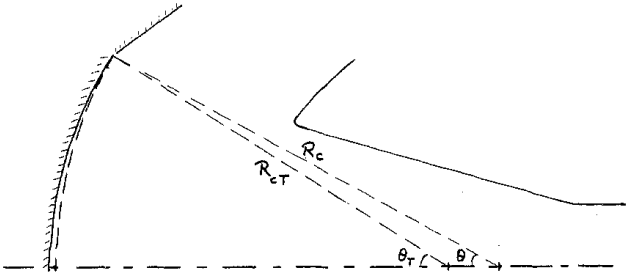
\includegraphics[width=0.8\linewidth]{figure/fig2}
	\caption{\small Modification of $ \theta $ and $ R_c $, as first described by Frost and Purl [6], to give the corrected design.}
	\label{fig2}
\end{figure}











\section{\textsc{Validation of the method}}


The Frost and Purl report [6] contains both dimensioned drawings of the guns and detailed and careful measurements of the exit beams. Thus it provides valuable independent material for testing the foregoing procedure: we enter their exit beam $ V, I $, and $ r_w $ assume that their working cathode current density was in fact the desired value. If the synthesis procedure can then rediscover (with acceptable accuracy) the gun that was actually used, and can do so for a substantial range of cases. then it is valid as a design procedure at least within that range.


Frost and Purl describe guns with perveance from $ 0.1 $ to $ 6\,\mu P$, and with area convergences from $ 36:1 $ to $ 300:1 $. The synthesis procedure did not perform satisfactorily on the $ 0.1\,\mu P $ design; apart from the problem of thermals at this low perveance, Frost and purl's center of cathode curvature was so close to the anode plane that the design could hardly be classified as a Pierce gun at all. For the $ 6\,\mu P $ case agreement was fair, but less than convincing: because of the deep curvature in relation to the spacing some arbitrary decisions have to be made on how to relate the model to the actual structure; since these decisions affect the agreement, they cloud the interpretation.


The three ``middle'' cases from the Frost and Purl report with perveance from 1.2 to 2.2, were then used to``calibrate'' the procedure by finding values of $ \Gamma $and $ k $ for the best overall fit. This fit was subjectively weighted, first in favor of accuracy on $ \theta $, and then on $ z_a $ as the two most important variables to control. The values $ \Gamma = 1.25 $ and $ k=0.905 $ so obtained were then used unchanged for three other cases as a test. All six cases are shown in Table \uppercase\expandafter{\romannumeral1}: the first three are the Frost and Purl cases, the fourth and fifth are an almost matched pair of relatively low-perveance designs by Litton and Varian respectively, and the sixth is a further design by Frost at high perveance.
 
Table \uppercase\expandafter{\romannumeral1} shows that, while this is not a precision calculation procedure, it does give a good first-trial value for all the major parameters over a wide range of conditions. The ``matched pair,'' cases 4 and 5, include both the best and worst agreement on $ \theta_T $. Exit-beam quality measurements have been made with beam testers on both these guns, and the profiles are compared in Fig.\ref{fig3}; this shows that the good agreement on $ \theta_T $ of case 4 is associated with excellent beam laminarity; case 5, on the other hand,has relatively poor agreement on $ \theta_T $, and a beam which becomes hot centered after passing through the waist.While this single comparison is far from conclusive,it certainly suggests that there is some merit in conforming to the calculated angle.

\begin{figure}[phtb]
	\centering
	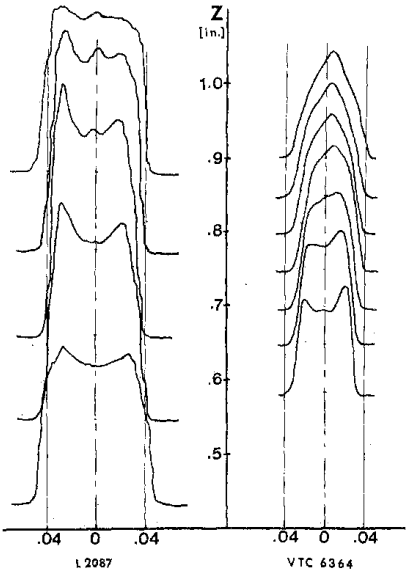
\includegraphics[width=0.6\linewidth]{figure/fig3}
		\caption{\small Comparison of exit-beam profiles for cases 4 and 5 of Table \uppercase\expandafter{\romannumeral1}. The VTC 6364 profiles copied from \ref{fig2} of [9], courtesy of Varian Associates, Inc.}
	\label{fig3}
\end{figure}



\begin{table*}[phtb]
	\centering
	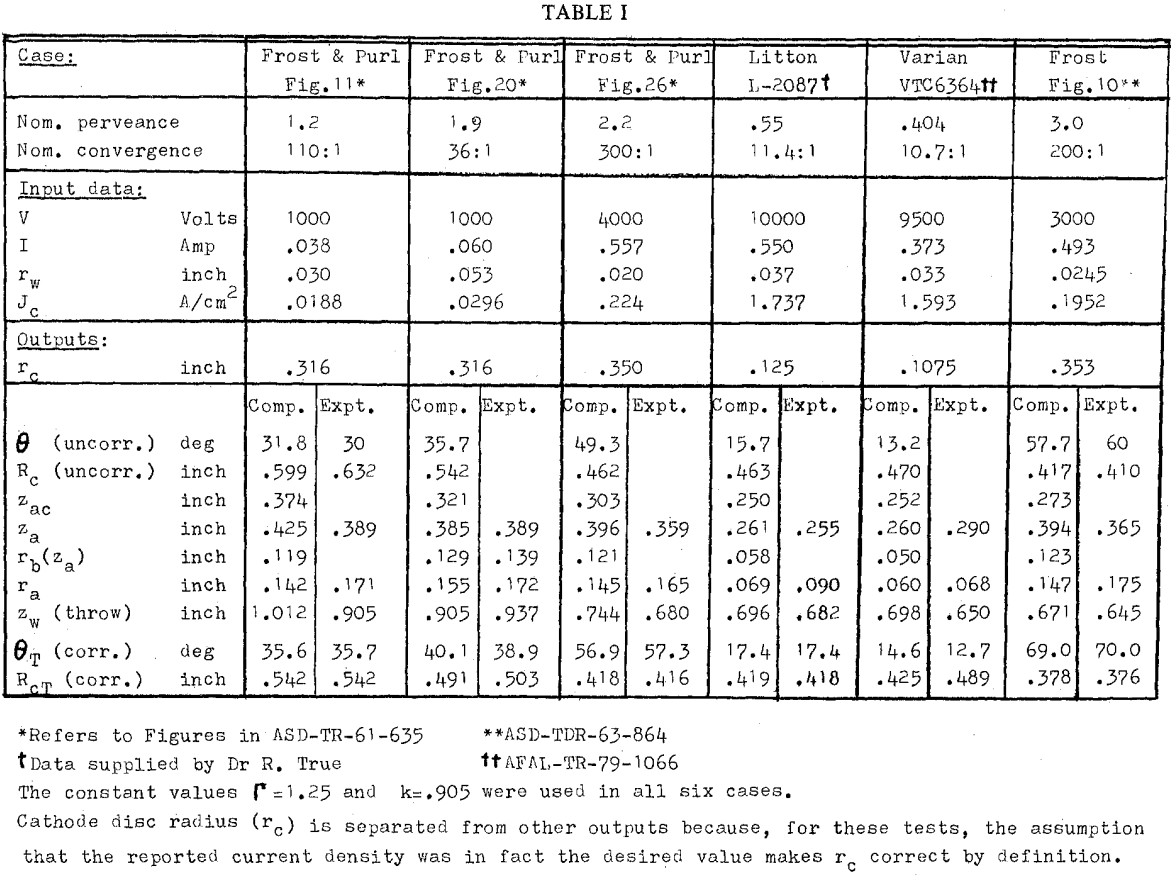
\includegraphics[width=0.9\linewidth]{figure/tab1}
	%	\caption{Fundamental mode axial electric field component on transverse cross section for phase, 2.5$ \pi $.}
	\label{tab1}
\end{table*}

















%Frost and Purl [67 found that the measured exit beam was larger in diameter and less uniform in current density than the beam expected from Pierce’s and Danielson’s theories. This was ascribed to a combination of spherical aberration and thermal-emission velocity effects. At the perveances mostly used for microwave tubes, the spherical aberration dominates, but the thermals can dominate low-perveance high-convergence cases.
%Frost and Purl found that an appropriate deepening of the cathode spherical curvature could compensate for these effects, at least when spherical aberration was dominant, producing an exit beam that was well defined and close to the intended diameter. This was later quantified by True [7] : new values 6T and R,T are defined by
%where k is an empirical constant less than unity,
%The similarity of(22)to Snell’s law in optics led True to call this “optical compensation.”
%For diode guns the value
%where k is an empirical constant less than unity
%The similarity of(22)to Snell's law in optics led True to call this ``optical compensation”
%For diode guns the value
%k=0.905
%appears to be a good compromise, as indicated by the test cases in Section IV. If the uncompensated diode half angle exceeds 64.8``(i.e, arc sin 0.905), the method becomes inapplicable because $\theta_T$ is then imaginary, but few guns are designed with such a large convergence. To illustrate the typical magnitude of this correction, Fig. 2 shows the case 8=30 0T=33: 5,k=0.905, drawn to scale.
%Thermal-Emission Velocity Effects
%The development so far has neglected these effects except to the extent that some part of the optical compensation, is applied to correcting for them. lo determine their importance we must run an analysis of the gun, using the D. R, and S procedure, first with a nominally zero cathode temperature and then with a realistic cathode temperature, the difference between the two cases will show how much of the waist radius is due to space charge and how much to thermals. This analysis can also be cared out on a programmable calculator using some closed-form approximations to the integrals in D, R, and S. If the thermal contribution is not too large, the synthesis procedure can then be rerun with the specified exit radius reduced by this amount to compensate. But if the thermal contribution is dominant. the synthesis procedure no longer works satisfactorily. Thus a Pierce gun for a CRT could probably not use this method. but most microwave tube guns fall within its scope.
%In making the D. R, and S analysis we use the uncorrected values $\theta$ and $R_c$, but in building the device we use the corrected 6r and r.r. with the expectation that the higher initial con vergence will compensate for the unanalyzed causes of excess divergence.
%A condensation of this Report was published by Frost, Purl, and H R. Johnson, ``Electron guns for forming solid beams of high Perveance and high convergence, Proc. I.R.E., Aug. 1962, pp. 1800--1807, but this paper does not include all the dimensional details necessary to test the procedure given here





In this connection, True has made the interesting observation that, among existing Litton gun designs, those whose angles conform to this theory are well behaved and relatively easy to build, while those which differ appreciably are notoriously ``cranky,'' both on his large ray-tracing program 181 and in construction. It appears that if one chooses the wrong angle, one may still be able to force reasonable performance by manipulation of the electrode shapes: but the penalty is poor. laminarity and a severe sensitivity to slight changes in the configuration.

The author is grateful to a reviewer for pointing out that test case \#6 theoretically fails at $ \eqref{eq:20} $ because the computed $ R_a $ is less than $ r_a $ (very slightly less). This had escaped notice because the author’s tests had all been run in Fortran on a large computer and on a TI 59 calculator; in both cases, the program continues past a ``square root of negative quantity.'' Fortran substitutes zero, while the TI 59 substitutes the root of the positive quantity, and in this case, the difference was hardly noticeable. (The two versions do not always give identical results in any case, because the differing levels of precision sometimes result in different numbers of iterations being performed to reach convergence.) Presumably, the reviewer programed the equations in Basic, which stops on a negative square root.




The conclusion is that for cases such as \#6 (high perveance and high convergence) the arbitrary factor 1.2 in $ \eqref{eq:18} $ may need to be adjusted; but if the program is forced (if necessary) to continue past a negative root, the remaining results can still be of useful accuracy.




The author has recently found that some low-convergence cases can also fail. Here the problem has been found to be that the first correction of $ \theta $ by the factor $ (\tan\phi_2/\tan\phi_1)^{1/2} $ is too strong, giving an interim value of $ r_b(z_a) $ less than $ r_w $, even thought he final value would be greater. The inverted UBS curve obviously cannot cope with $ R $ less than unity, and the program either stops or begins to diverge. Changing the exponent from $ \frac{1}{2} $ to $ \frac{1}{4} $ has been found effective in restoring stability, at the cost of a few extra iterations.




\renewcommand{\thefootnote}{{$ ^* $}}
\section*{\textsc{References\footnote{Please refer to the \hyperref{https://ieeexplore.ieee.org/document/1481431/}{}{}{original article} to get more information.}}}







%\newpage
%\enlargethispage{-6.5cm}




%\begin{table}[htbp]
%	\caption{盒型窗计算参数}
%	\centering
%	\begin{tabular}{cc}
%		\toprule
%		Parameters & Dimension($ \mu $m) \\ \midrule
%		$ a $    &         520         \\
%		$ b $    &         254         \\
%		$ p $    &         240         \\
%		$ w $    &         100         \\
%		$ g $    &         40          \\
%		$ h $    &         113         \\
%		$ d $    &         115         \\
%		$ t $    &         60          \\ \bottomrule
%	\end{tabular}
%	\label{tab:1}
%\end{table}

%\newpage
%\enlargethispage{-6.5cm}

%\section*{Reference\footnote{注:本文为译文,相关参考文献见原文。原文文献信息如下:\href{http://ieeexplore.ieee.org/document/7426768/}{H-Plane and E-Plane Loaded Rectangular
%			Slow-Wave Structure for Terahertz TWT Amplifier,IEEE TRANSACTIONS ON ELECTRON DEVICES, VOL. 63, NO. 4, APRIL 2016}\\(翻译人:李胜明)}}


\end{document}